% Poster Coefis 2019-2020

%--------------------------------------------------------------------
% PACKAGES AND OTHER DOCUMENT CONFIGURATIONS
%--------------------------------------------------------------------

\documentclass[a0,portrait]{a0poster} % Tamaño del póster en A0
    %Columnas
\usepackage{multicol} % Permite la creación de columnas en el póster
\columnsep=100pt % Separación entre las columnas
%\columnseprule=3pt % Línea de separación entre columnas
    %Paleta de colores
\usepackage[svgnames]{xcolor} % Gama de colores http://www.latextemplates.com/svgnames-colors
    %Fuente y lenguaje
\usepackage{times} % Fuente Times New Roman
\usepackage[utf8]{inputenc} % Codificación de caracteres para poder usar tildes y otros caracteres especiales
\usepackage[spanish]{babel} % Establece el idioma del documento en español
    %Texto
\usepackage[document]{ragged2e} % Alineación del texto
    %Imágenes
\usepackage{graphicx,type1cm, lettrine} % Incluir imágenes
\usepackage[font=small,labelfont=bf]{caption} % Personalización de los títulos de las imágenes
\usepackage{wrapfig} % Permite colocar imágenes con texto alrededor
\usepackage{subfigure} % Creación de subfiguras
\usepackage{setspace} % Espaciado de líneas personalizado
\usepackage[left=2cm,right=2cm,top=2cm,bottom=2cm]{geometry} % Márgenes del documento

%Matemáticas
\usepackage{amsfonts, amsmath, amsthm, amssymb} % Paquete de matemáticas
\usepackage{esvect} % Permite usar vectores
    %Color
\usepackage{tcolorbox} % Personalización de cajas de texto
\usepackage{xcolor} % Permite el uso de colores
\usepackage{transparent} % Permite la transparencia
\usepackage{float} % Personalización de la ubicación de imágenes

%--------------------------------------------------------------------- 
% Fondo de pantalla configuración
%---------------------------------------------------------------------
\usepackage[pages=all]{background} % Permite establecer una imagen de fondo para todo el documento
%La opción pages puede ser all (para todo el documento) o some, para algunas partes del documento
% Configuración de la imagen de fondo
\backgroundsetup{
 scale=1, % Escala de la imagen
 color=black, % Fondo a usar para transparencia
 opacity=1, % Nivel de transparencia
 angle=0, % En caso de querer una rotación
 contents={%
  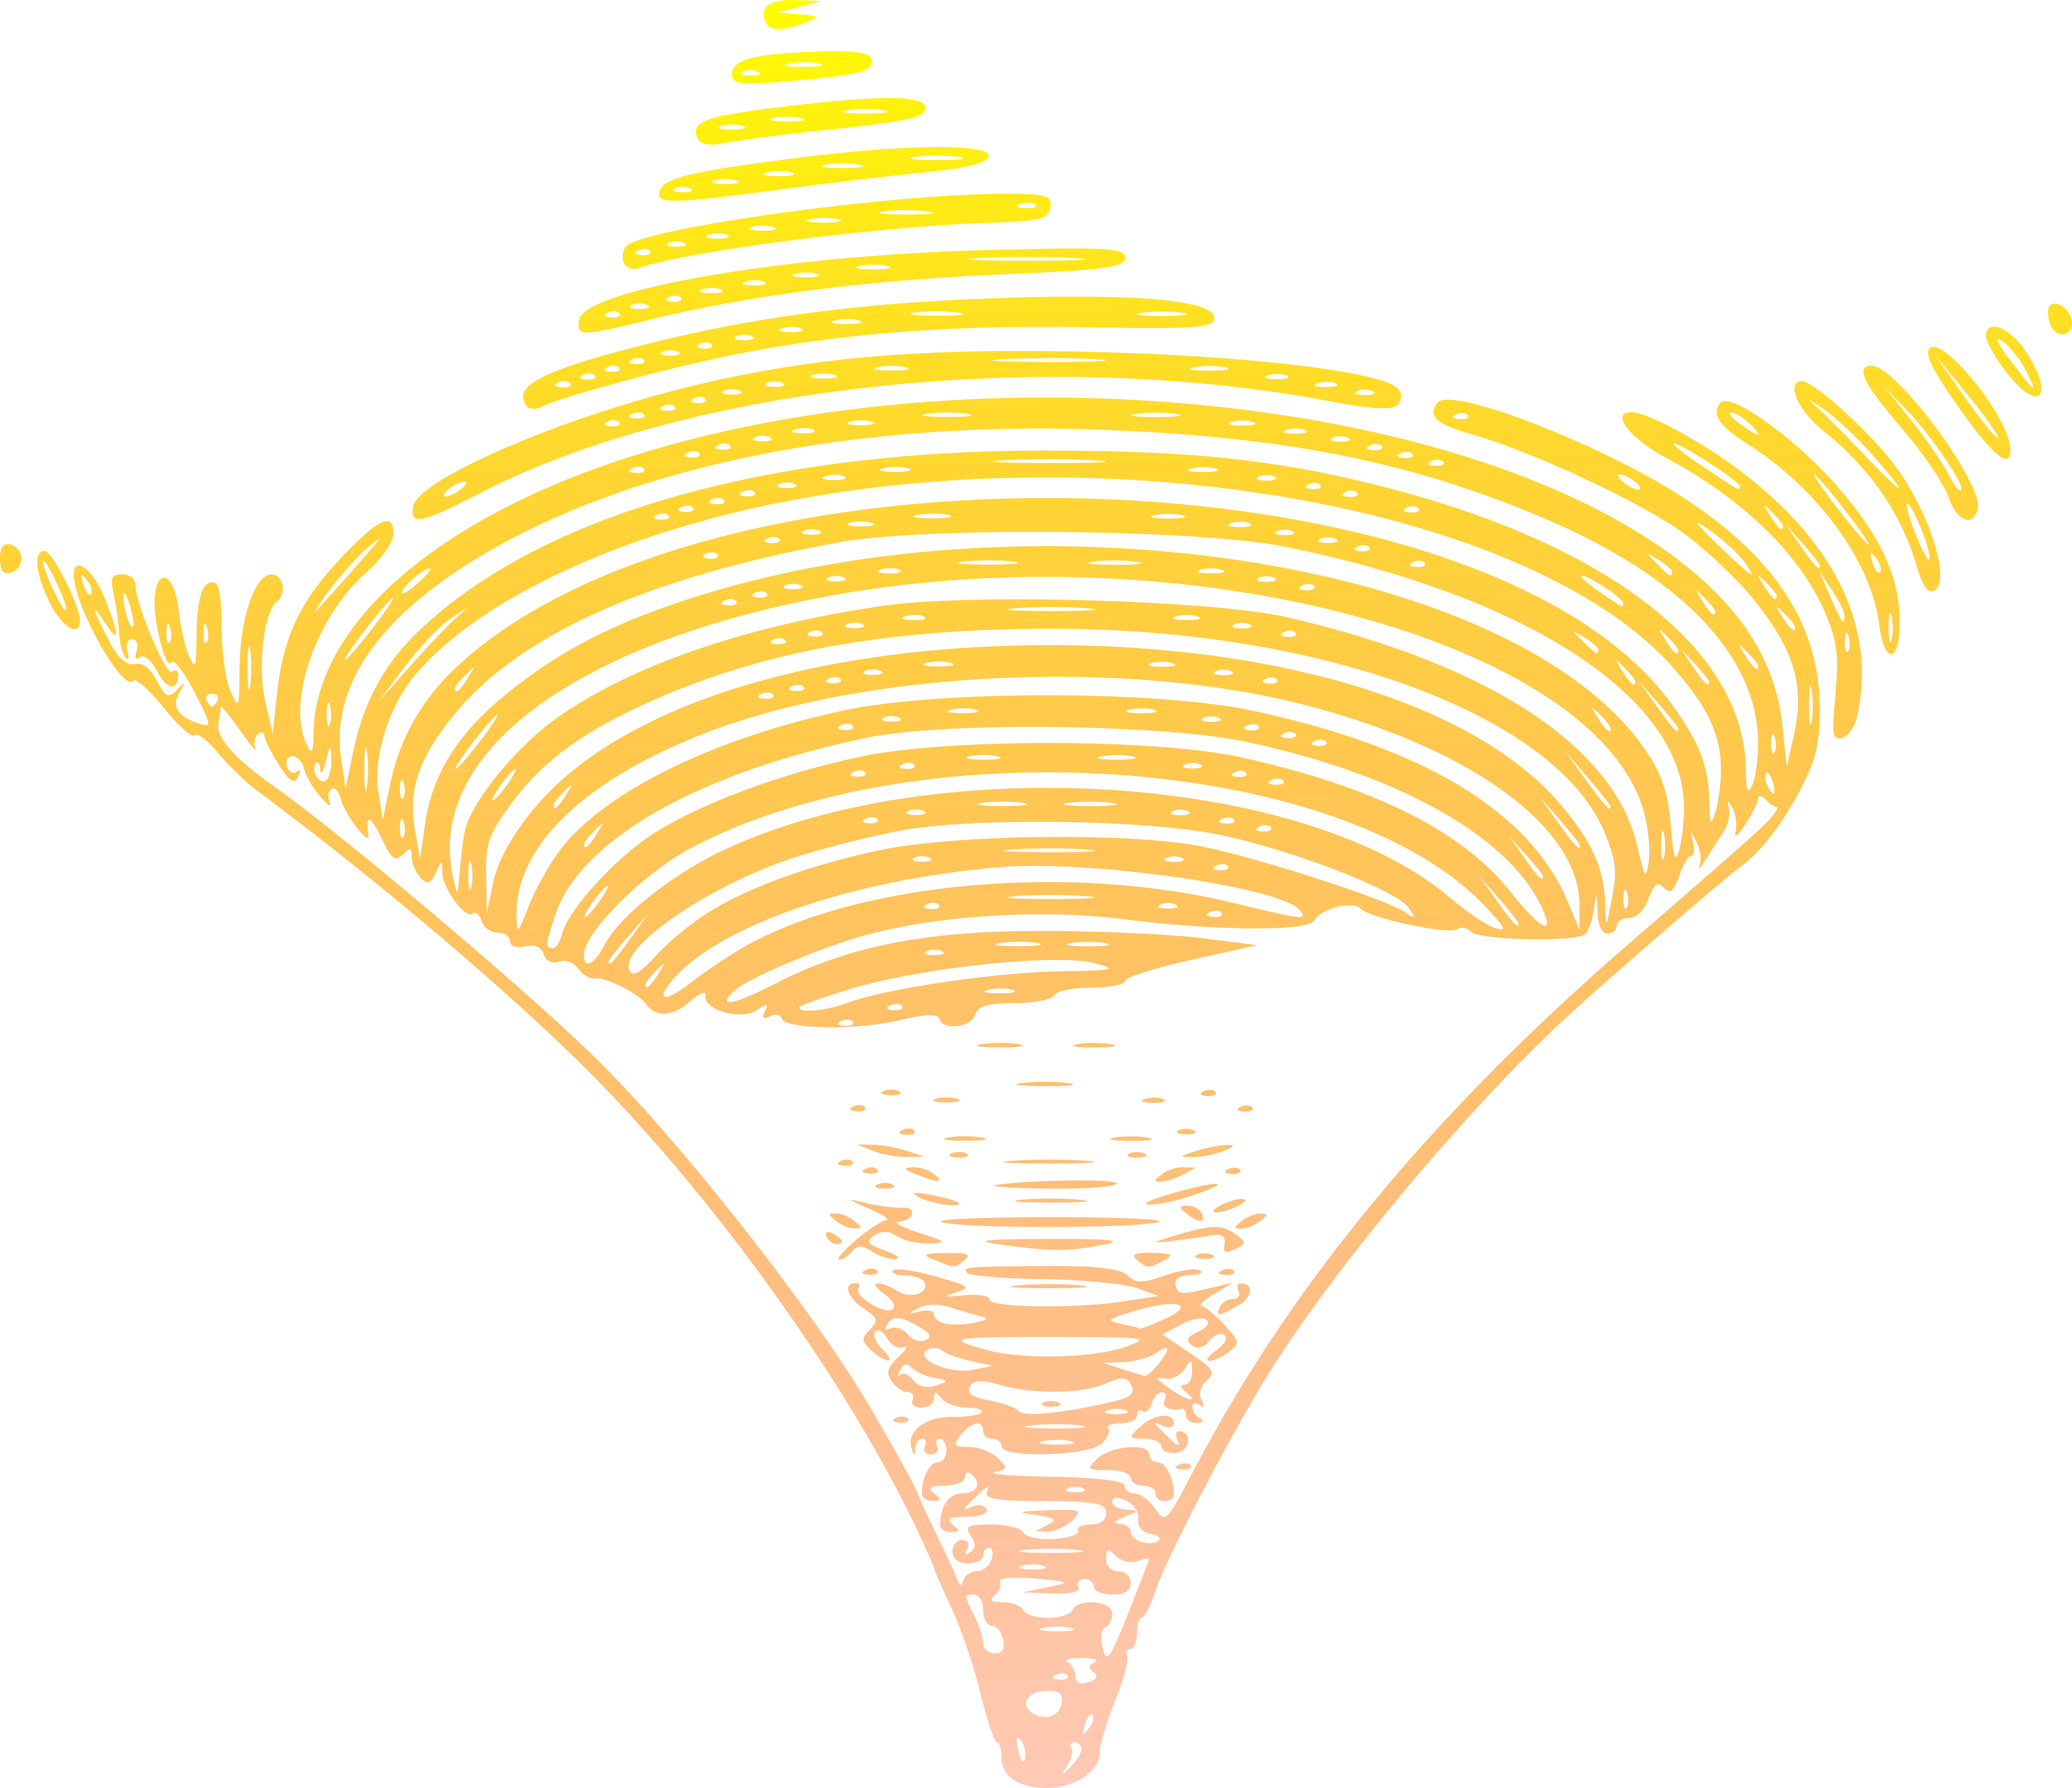
\includegraphics[width=150cm,height=120cm]{media/Fondo_poster.png}% Nombre de la imagen a utilizar como fondo
 }%
}

%---------------------------------------------------------------------
% Encabezado del título.
%---------------------------------------------------------------------
\title{\veryHuge Acción de Einstein-Hilbert} % Título del póster
\author{\textsc{\huge Juan José Fernández Morales}} % Autor del póster
\date{} % No aparece fecha


\begin{document}

\maketitle
\thispagestyle{empty}

%---------------------------------------------------------------------
%   Abstrac
%---------------------------------------------------------------------

\begin{abstract}\centering \fontsize{36}{40} \selectfont
    La acción es una magnitud física que surge con la formulación de la mecánica analítica del siglo XVIII y el principio de Hamilton, postulado que se mantiene vigente en la mecánica relativista. Este póster contiene dos partes: en la primera se introduce al lector en el estudio de esta magnitud y sus posibles aplicaciones, y en la segunda se describe la acción de Einstein-Hilbert y la obtención de las ecuaciones de campo de Einstein.
    
\end{abstract}

\vspace{25pt}\textbf{}

\begin{multicols}{2}
%---------------------------------------------------------------------
% Acción
%---------------------------------------------------------------------

\section*{\centering La acción}

\justify{En Física, la acción $(S)$ se expresa como un funcional que define el producto de la energía y el tiempo empleados en un cierto proceso. Por tanto, se puede deducir que las unidades de la acción son $[Energ\acute{i}a]\cdot[tiempo]$, en el Sistema Internacional de Unidades $(J\cdot s)$.}

\vspace{8pt}\textbf{}

\begin{equation}
    \label{Eq: 1}
    S_{AB} = \int_A^B(E_c - E_p)dt
\end{equation}

\begin{center}\small
    Expresión común de la acción en mecánica clásica de un sistema conservativo donde  
    
    $E_c$ y $E_p$ representan la energía cinética y la energía potencial respectivamente.
\end{center}

\vspace{50pt}\textbf{}

\justify{\textbf{Observación:} La constante de Planck $(h \simeq 6.62607015\cdot10^{-34}J\cdot s)$ presenta las mismas unidades que la acción, por eso el lector se puede encontrar que a esta constante también se le denomina como <<\textit{cuanto de acción}>> o <<\textit{unidad natural de la acción}>>.}

%---------------------------------------------------------------------
% FUNCIONAL
%---------------------------------------------------------------------

\subsection*{La acción como funcional}

\justify{Un funcional se puede definir de varias formas, normalmente depende del campo de las matemáticas en el el que se le esté haciendo uso, para este trabajo resulta suficiente si se describe como una función $(\mathcal{F})$ cuyo argumento es otra función $(f)$, y se denota como:}

\begin{align*}
    \mathcal{F}: D_f &\rightarrow D_\mathcal{F} \\
    f &\mapsto \mathcal{F}[f]
\end{align*}

\justify{Donde $D_f$ y $D_\mathcal{F}$ son los dominios de $f$ y de $\mathcal{F}$ respectivamente.}

\justify{Nuestra magnitud escalar se encuentra dentro de un subconjunto de funcionales reales que se caracterizan por estar expresados con una integral. Al integrando de la acción se le denomina lagrangiano ($L$) cuando el integrador es temporal o densidad lagrangiana $(\mathcal{L})$ cuando el integrador es espacio-temporal \cite{Tensor1}\cite{Tensor4}.}

\begin{align}
    \label{Eq: 2}
    S[\textbf{q}(\cdot)] &= \int_T L\left(\textbf{q}(t), \partial_t \textbf{q}(t), t \right) dt \\
    \label{Eq: 3}
    S[\phi(\cdot)] &= \int_M \mathcal{L}(\phi(\textbf{x}), \partial\phi(\textbf{x}), \partial\partial \phi(\textbf{x}), \textbf{x}) d^4x
\end{align}

\justify{Donde $\textbf{q} = (q_1, \cdots, q_N)$ son las coordenadas generalizadas, donde $d^4x = dxdydzd(ct)$.}

\justify{\textbf{Observación}: Si se compara la ecuación (\ref{Eq: 2}) con la (\ref{Eq: 1}) se puede observar que el lagrangiano de un sistema clásico conservativo viene dado por la diferencia de las energías cinética y potencial $(L_{cl\acute{a}sico} = E_c - E_p)$.}

%---------------------------------------------------------------------
% PRINCIPIOS
%---------------------------------------------------------------------

\section*{\centering Principio de mínima... de Hamilton}

\justify{El principio de Hamilton, o principio de acción estacionaria, es un postulado que relaciona la acción con la dinámica de un sistema físico, y afirma que la trayectoria que describen los cuerpos es aquella que hace la acción invariante. Matemáticamente el principio se puede expresar como:}

\begin{equation}
    \label{Eq: principio}
    \delta S = 0
\end{equation}

\justify{El cálculo variacional es el campo de las matemáticas que aborda esta tipología de problemas, las soluciones denominadas ecuaciones de Euler-Lagrange resultan ser, a su vez, las expresiones del movimiento de los cuerpos que conforman el sistema físico. Se aplica el principio a las ecuaciones (\ref{Eq: 2}) y (\ref{Eq: 3}):}

\begin{align}
    \label{Eq: EL1}
    0 &= \delta \int_T L\left(\textbf{q}(t), \partial_t \textbf{q}(t), t \right) dt \rightarrow \frac{d}{dt}\left(\frac{\partial L}{\partial (\partial_t q_i)} \right) - \frac{\partial L}{\partial q_i} = 0\\
    \label{Eq: EL2}
    0 &= \delta \int_M \mathcal{L}(\phi(\textbf{x}), \partial\phi(\textbf{x}), \partial\partial \phi(\textbf{x}))d^4x \rightarrow \partial_\mu\left(\frac{\partial \mathcal{L}}{\partial(\partial_\mu \phi)}\right) - \frac{\partial \mathcal{L}}{\partial \phi} = 0
\end{align}

\justify{\textbf{Cuidado:} en la expresión (\ref{Eq: EL2}) se emplea la notación de Einstein, convenio que se emplea de aquí en adelante.}

\end{multicols}

%---------------------------------------------------------
%   La acción del universo
%---------------------------------------------------------
\vspace{15pt}\textbf{}

\section*{\centering Acción del Universo}

\begin{center}
    \fontsize{32}{40} \selectfont Se suele describir la acción del universo $(S)$ como suma de la acción de Einstein-Hilbert $(S_{EH})$, la acción cosmológica $(S_{cosmo})$ y la acción material $(S_{matter})$. 
\end{center}

\vspace{5pt}\textbf{}

%---------------------------------------------------------
%   Tercera Parte
%---------------------------------------------------------

\begin{multicols}{2}
\subsection*{Acción de Einstein-Hilbert}

\justify{Se propone que la acción relacionada con la dinámica de la gravedad tiene que presentar una densidad lagrangiana escalar que esté relacionada con la curvatura, en este caso del espacio tiempo \cite{Relatividad1}\cite{Tensor2}. La acción de Einstein-Hilbert satisface estos criterios y se describe como:}

\begin{equation}
    S_{EH} = \frac{c^4}{16\pi G}\int d^4x\sqrt{-g}g^{\mu\nu}R_{\mu\nu}
\end{equation}

\justify{Donde $c$ y $G$ son las constantes de la velocidad de la luz y de la gravitación universal respectivamente, necesarias para mantener las unidades, g es el determinante del tensor métrico, $g^{\mu\nu}$ es el tensor métrico contravariante y $R_{\mu\nu}$ es el Tensor de Ricci.}

\justify{Al aplicar el principio de acción estacionaria se queda la variación de un producto de tres términos ($\sqrt{-g}$, $g^{\mu\nu}$, $R_{\mu\nu}$). La variación del primero se obtiene con la fórmula de Jacobi para la derivada de un determinante ($\delta\sqrt{-g} = \frac{-1}{2}\sqrt{-g}g_{\mu\nu}\delta g^{\mu\nu})$ y al último, si se integra tras emplear la identidad de Palatini \cite{Tensor2} se obtiene un término de frontera que no afecta a las expresiones del movimiento, por lo que se puede obviar.}

\begin{equation}
    \delta S_{EH} = \int d^4x\sqrt{-g}\left(\frac{-1}{2}g^{\mu\nu}R_{\mu\nu}g_{\mu\nu} + R_{\mu\nu} \right)\delta g^{\mu\nu} = 0
\end{equation}

\justify{Si se emplea el lema fundamental del cálculo variacional y se sustituye la contracción $g^{\mu\nu}R_{\mu\nu}$ por el Escalar de Ricci ($R$) queda:}

\begin{equation}
    \label{Eq: 9}
    R_{\mu\nu} -\frac{1}{2}Rg_{\mu\nu} = 0
\end{equation}

\justify{Al término de la izquierda se le conoce como Tensor de Einstein $(E_{\mu\nu})$ y las soluciones a esta ecuación son las denominadas ecuaciones de Einstein en el vacío $(R_{\mu\nu} = 0)$ \cite{Relatividad2}.}

\subsection*{Acción cosmológica}

\justify{La acción cosmológica se propone con el fin de modificar la expresión (\ref{Eq: 9}), para eso se le añade la constante cosmológica $(\Lambda$) a la integral \cite{Tensor3}. Se puede observar que su variación solo depende de una componente ya conocida $(\sqrt{-g}$):}

\begin{equation}
    \label{Eq: cosmo}
    S_{cosmo} = \frac{c^4}{16\pi G}\int d^4x\sqrt{-g}\left(-2\Lambda\right)
\end{equation}

\justify{Esta modificación consigue un término extra ($\Lambda g_{\mu\nu}$) en las ecuaciones de evolución, el signo de este parámetro resulta crucial para definir la evolución del universo; actualmente las observaciones astronómicas acotan la constante a un valor positivo pero menor o igual que $10^{-46}km^{-2}$ por lo que actualmente se afirma una expansión acelerada del universo.}

\subsection*{Acción material}
\justify{Finalmente, la acción material trata de la resultante del conjunto de acciones de campos clásicos (ejemplo: la acción del campo electromagnético $(S_{Maxwell}$):}

\begin{equation}
    S_{matter} = \int d^4x \sqrt{-g} \mathcal{L}_{matter}
\end{equation}

\justify{La variación de esta acción dependerá de la forma de la densidad lagrangiana ($\mathcal{L}_{matter}$), análogo a la expresión (\ref{Eq: 3}), pero se puede asegurar que su variación tiene que tener la forma de un tensor variante (para mantener el comportamiento escalar de la acción) al que se denominará Tensor energía-impulso $(T_{\mu\nu})$ \cite{Relatividad1}.}

\begin{equation}
    \delta S_{matter} = \int d^4x \sqrt{-g} \frac{-1}{2}T_{\mu\nu} \delta g^{\mu\nu}
\end{equation}
\end{multicols}

%-------------------------------------------------------
% Lo que me gustaría añadir
%-------------------------------------------------------
\section*{\centering Ecuaciones de campo de Einstein}

\begin{center} Con el principio de Hamilton se puede obtener las ecuaciones de campo de Einstein, éstas describen la geometría del espacio-tiempo debido a la materia que se encuentra en él.
\end{center}

\begin{equation*}
    S = \int d^4x \sqrt{-g}\left[\frac{c^4}{16\pi G}\left(g^{\mu\nu}R_{\mu\nu} - 2\Lambda \right) +  \mathcal{L}_{matter} \right] \rightarrow \delta S = \int d^4x \sqrt{-g}\left[\frac{c^4}{16\pi G}\left(R_{\mu\nu} - \frac{1}{2}R g_{\mu\nu} + \Lambda g_{\mu\nu} \right) - \frac{1}{2}T_{\mu\nu}  \right]\delta g^{\mu\nu} = 0 
\end{equation*}

\begin{equation*}
    \frac{c^4}{16\pi G}\left(R_{\mu\nu} - \frac{1}{2}R g_{\mu\nu} + \Lambda g_{\mu\nu} \right) - \frac{1}{2}T_{\mu\nu} = 0 \leftrightarrow \mathbf{ R_{\mu\nu} - \frac{1}{2}R g_{\mu\nu} + \Lambda g_{\mu\nu} = \frac{8\pi G}{c^4}T_{\mu\nu} }
\end{equation*}

%-------------------------------------------------------
% Bibliografía y logo 
%-------------------------------------------------------

\begin{multicols}{2}
\vspace{20pt}\textbf{}
\small{
\begin{thebibliography}{6}
\bibitem{Relatividad1}
Anthony Zee.
\textit{Einstein Gravity in a Nutshell}.
(PRINCETON UNIVERSITY PRESS), 2013. Chapter VI.

\bibitem{Relatividad2}
Fernando H. Pérez Hernández.
\textit{Relatividad General}.
2019. Chapter VI.

\bibitem{Tensor1}
Rodolfo Alexander Fiaz Sanchez.
\textit{Mecánica Analítica: Notas de Clase}
2012. Chapter XVIII.

\bibitem{Tensor2}
Javier Garcia (Canal de Youtube).
\text{54 - Curso de Relatividad General [Acción Hilbert Einstein 3]}, 2019.

\bibitem{Tensor3}
Hanoch Gutfreund y Jürgen Renn.
\textit{El camino hacia la relatividad}.
(PRINCETON UNIVERSITY PRESS), 2017.

\bibitem{Tensor4}
L.D. Landau y E. M. Liftshitz
\text{Mecánica Volumen 1}.
(EDITORIAL REVERTÉ), 1994.
\end{thebibliography}}

\begin{figure}[H]
    \centering
    
\includegraphics[scale = 0.8]{media/logo_coefis.png}
\end{figure}

\end{multicols}

\end{document}

